% \section{System Call}

\begin{frame}[fragile]{System Calls}
	When a user program needs to do something privileged, it \textbf{calls a system call}. A system call is a special kind of trap.
	\begin{figure}[H]
		\centering
		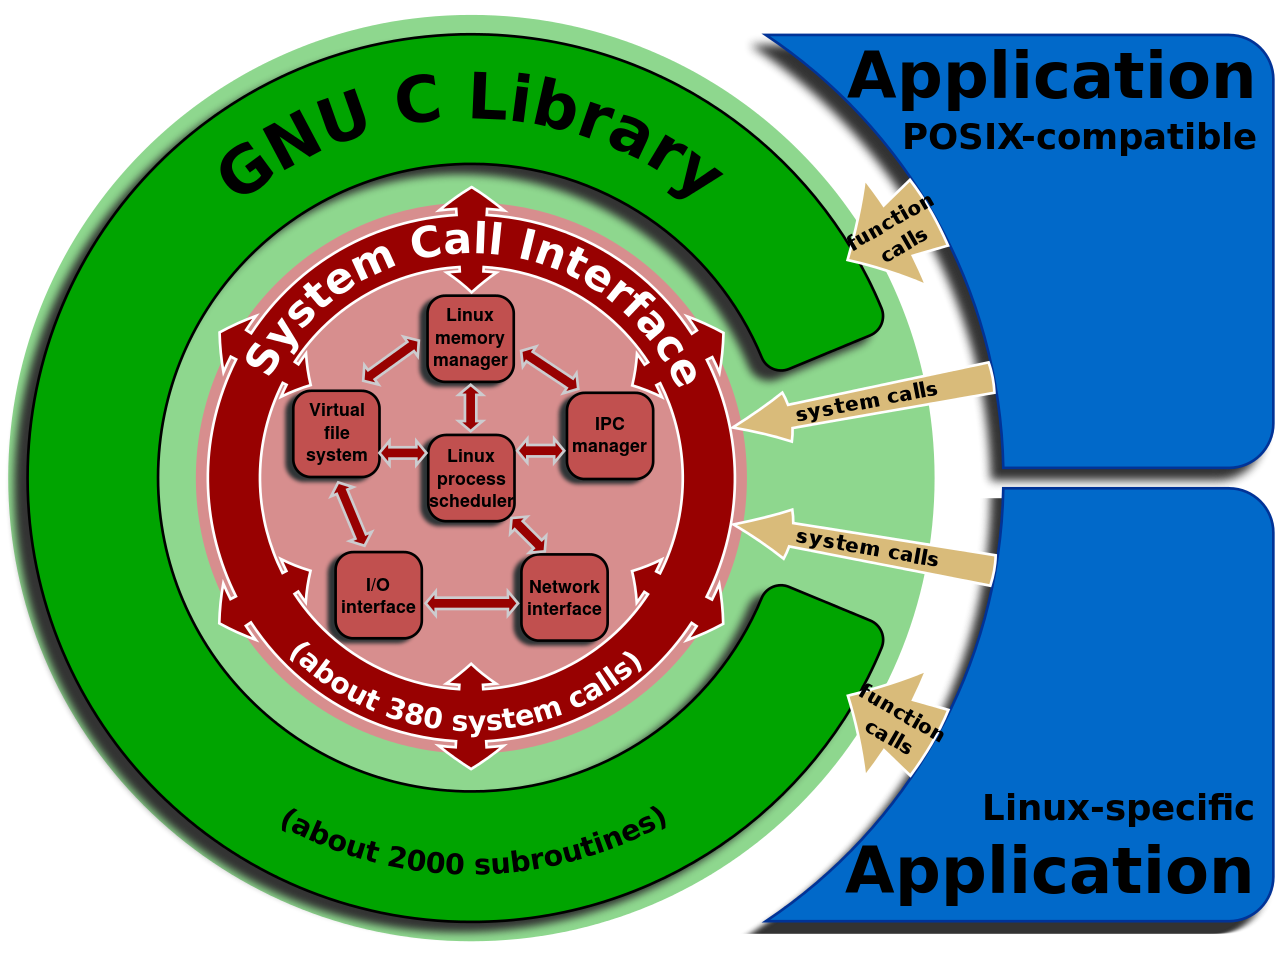
\includegraphics[width=0.5\textwidth]{day3/img/syscall.png}
	\end{figure}

\end{frame}

\begin{frame}[fragile]{10k meter view of kernel code (revised)}
	\begin{minted}[fontsize=\scriptsize,highlightlines={10-12}]{c}
void processEvent(event) {
    switch (event.type) {
        case NETWORK_COMMUNICATION:
            NetworkManager.handleEvent(event);
            break;
        case SEGMENTATION_FAULT:
        case INVALID_MODE:
            ProcessManager.handleEvent(event);
            break;
        case SYSTEM_CALL:
            SystemCallManager.handleEvent(event);
            break;
        // ...
    }
}
    \end{minted}
\end{frame}

\begin{frame}[fragile]{System Call Handler}
	\begin{figure}[H]
		\centering
		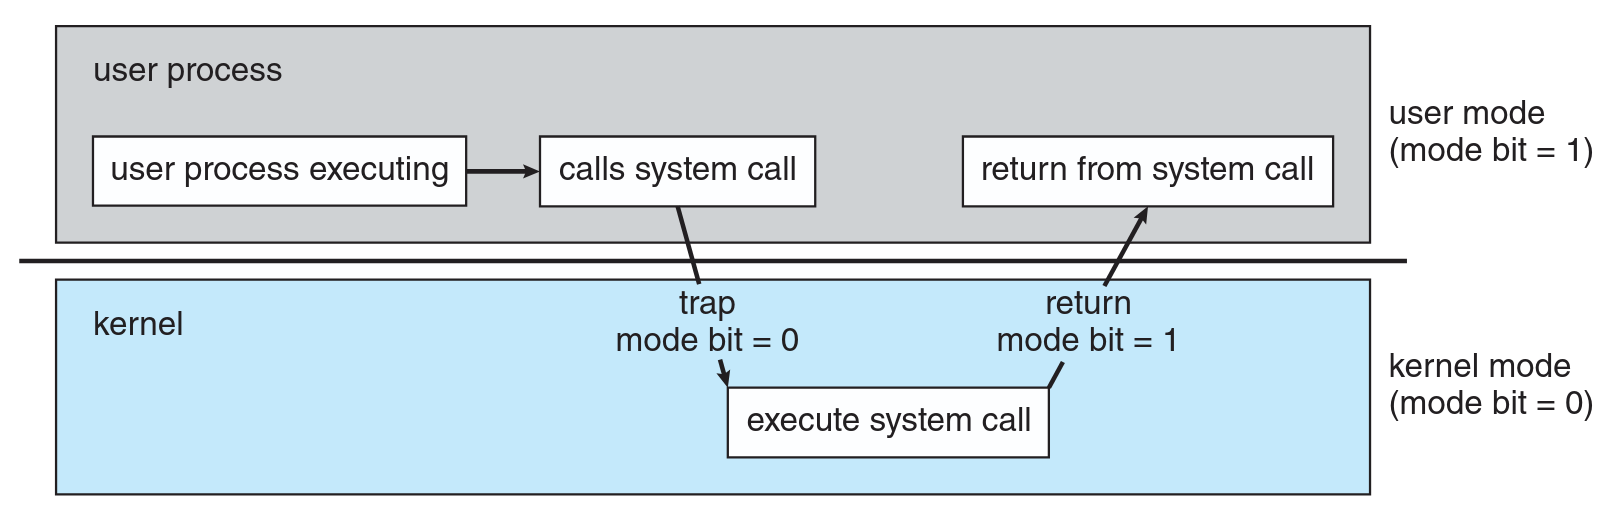
\includegraphics[width=\textwidth]{day3/img/interrupt.png}
	\end{figure}
\end{frame}

\begin{frame}[fragile]{Timers}
	\begin{itemize}
		\item The OS must keep control of the CPU
		      \begin{itemize}
			      \item Programs cannot get stuck in infinite loop and lock up the computer
			      \item Programs cannot gain an unfair share of the computer
		      \end{itemize}
		\item One way in which the kernel retrieves
		      control is when an interrupt occurs
		\item To make sure that an interrupt will occur reasonably soon, we can use a timer
	\end{itemize}
\end{frame}

\begin{frame}[fragile]{10k meter view of kernel code (revised)}
	\begin{minted}[fontsize=\scriptsize,highlightlines={3-5}]{c}
void processEvent(event) {
    switch (event.type) {
        case TIMER_INTERRUPT:
            TimerManager.handleEvent(event);
            break;
        // ...
        case SYSTEM_CALL:
            SystemCallManager.handleEvent(event);
            break;
        // ...
    }
}
    \end{minted}
\end{frame}
